\section{Expected Benefits}
\label{chap:improvement:benefits}

\mnote{Benefits overview}
We expect several benefits from the \commonalities approach in comparison to defining networks of transformations for preserving consistency between multiple models.
First, we claim to achieve better \emph{comprehensibility} by making common concept explicit rather than implicitly encoding them in consistency relations.
Second, we mitigate trade-offs between specific quality properties, in particular correctness and reusability, of the defined transformation networks.
Finally, it promises to reduce the specification effort at least in specific scenarios.
While the improvement in comprehensibility is only a claim, we discuss why we expect the benefits of mitigating trade-offs and reducing specification effort in the following.


\subsection{Improving Correctness and Reusability}
\label{chap:improvement:benefits:properties}

\mnote{Correctness and reusability}
We have discussed the benefits of the \commonalities approach regarding correctness guarantees in \autoref{chap:improvement:commonalities:tree}.
This results from a transformation network defined with the \commonalities approach being intended to induce a tree topology.
At the same time, a network defined by \commonalities also improves reusability, although the network forms a tree and reusability is actually a benefit of dense graphs, as discussed in \autoref{chap:classification:topologies:effects}.

\begin{figure}
    \centering
    \begin{minipage}[b]{0.49\columnwidth}
        \centering
        \newcommand{\hmmdistance}{3.6em}
\newcommand{\vmmdistance}{2.4em}

\begin{tikzpicture}[
    mm/.style={schematic metamodel},
]

\node[mm] (full_left) {};
\node[mm, above right=\vmmdistance and \hmmdistance of full_left.center, anchor=center] (full_top) {};
\node[mm, below right=\vmmdistance and \hmmdistance of full_left.center, anchor=center] (full_bottom) {};
\node[mm, right=2*\hmmdistance of full_left.center, anchor=center] (full_right) {};
\node[mm, below left=\vmmdistance and \hmmdistance of full_left.center, anchor=center] (full_bottomleft) {};

\draw[transformation] (full_left) -- (full_top);
\draw[transformation] (full_left) -- (full_right);
\draw[transformation] (full_left) -- (full_bottom);
\draw[transformation] (full_top) -- (full_right);
\draw[transformation] (full_top) -- (full_bottom);
\draw[transformation] (full_right) -- (full_bottom);
\draw[transformation] (full_left) -- (full_bottomleft);
\draw[transformation] (full_bottom) -- (full_bottomleft);
\draw[transformation] (full_top) to[bend right=30] (full_bottomleft);
\draw[transformation] (full_bottomleft) .. controls ++(1*\hmmdistance, -0.8*\vmmdistance) and ([yshift=-1.5*\vmmdistance]full_right.south) .. (full_right);

\end{tikzpicture}
        \subcaption{Complete Graph}
        \label{fig:improvement:topologies:complete}
    \end{minipage}
    \hfill
    \begin{minipage}[b]{0.49\columnwidth}
        \centering
        \newcommand{\hmmdistance}{3.6em}
\newcommand{\vmmdistance}{2.4em}

\begin{tikzpicture}[
    conceptmm/.style={schematic conceptmetamodel},
    concretemm/.style={schematic metamodel},
]

\node[conceptmm, right=4*\hmmdistance of full_left.center, anchor=center] (tree_left) {};
\node[conceptmm, above right=\vmmdistance and \hmmdistance of tree_left.center, anchor=center] (tree_top) {};
\node[concretemm, below right=\vmmdistance and \hmmdistance of tree_left.center, anchor=center] (tree_bottom) {};
\node[concretemm, right=2*\hmmdistance of tree_left.center, anchor=center] (tree_right) {};
\node[concretemm, below left=\vmmdistance and \hmmdistance of tree_left.center, anchor=center] (tree_bottomleft) {};

\draw[transformation] (tree_left) -- (tree_top);
\draw[transformation] (tree_left) -- (tree_bottom);
\draw[transformation] (tree_left) -- (tree_bottomleft);
\draw[transformation] (tree_top) -- (tree_right);

\end{tikzpicture}
        \vspace{1em}
        \subcaption{\commonalities Tree}
        \label{fig:improvement:topologies:tree}
    \end{minipage}
    \caption[Benefit of \commonalities regarding quality trade-offs]{Dense graphs as an extreme of transformation network topologies in comparison to the tree topology of a \commonalities specification. Nodes depict metamodels and edges depict transformations. In a \commonalities specification, leaves represent \concretemetamodels whereas inner nodes represent \conceptmetamodels. Adapted from~\owncite[Fig. 4]{klare2019models}.}
    \label{fig:improvement:topologies}
\end{figure}

\mnote{Extreme topologies}
\autoref{fig:improvement:topologies} depicts the topology extremes of complete graphs and trees.
In the tree topology of a \commonalities specification, the \concretemetamodels are represented by leaves of the tree, whereas the inner nodes represent the \conceptmetamodels.
This depiction is reduced to metamodels rather than \metaclasses and \commonalities, as discussed in \autoref{chap:improvement:commonalities:tree} for the tree structure, but would be the same if considered at the level of \metaclasses.

\mnote{Reusability in trees}
In \autoref{chap:classification:topologies:effects}, we have discussed that reusability is improved in transformation networks inducing a dense or even complete graph, as a transformation exists for each metamodel pair and thus the transformations for any subset of the metamodels can be reused in other transformation networks relating a different set of metamodels.
Having a tree topology, only subtrees can be reused, as otherwise consistency between some of the metamodels cannot be preserved because it was expressed transitively via transformations across metamodels that are not part of the subset to be reused.

\mnote{Reusability in \commonalities}
This is, however, different for a network defined with the \commonalities approach.
Although it forms a tree, the \concretemetamodels to be reused in other networks are only leaves of that tree.
Any subset of them can be reused without loosing transformations that preserve consistency between them by also reusing all \conceptmetamodels on each path between two of the \concretemetamodels to reuse.
Since \conceptmetamodels and their instances only represent auxiliary artifacts for describing consistency relations and their preservation, it is not a drawback that they have to be reused. % in other transformation networks.

\mnote{Trade-off mitigation}
For these reasons, defining consistency with the \commonalities approach has the same benefits regarding correctness (and also other maintainability properties as discussed in \autoref{chap:classification:topologies:effects}) as defining a transformation network with tree topology, but at the same improves reusability by allowing any subset of the \concretemetamodels and the specification of consistency between them to be reused.
The central limitation of the approach is regarding completeness, since the manifestation relations between \metaclasses and \commonalities must induce a specific tree structure, namely a consistency relation tree according to \autoref{def:relationtree}, to actually provide the benefits regarding correctness.
It is part of our evaluation in \autoref{chap:commonalities_evaluation} to validate the achievability of that property in practical scenarios.

% \begin{figure}
%     \centering
%     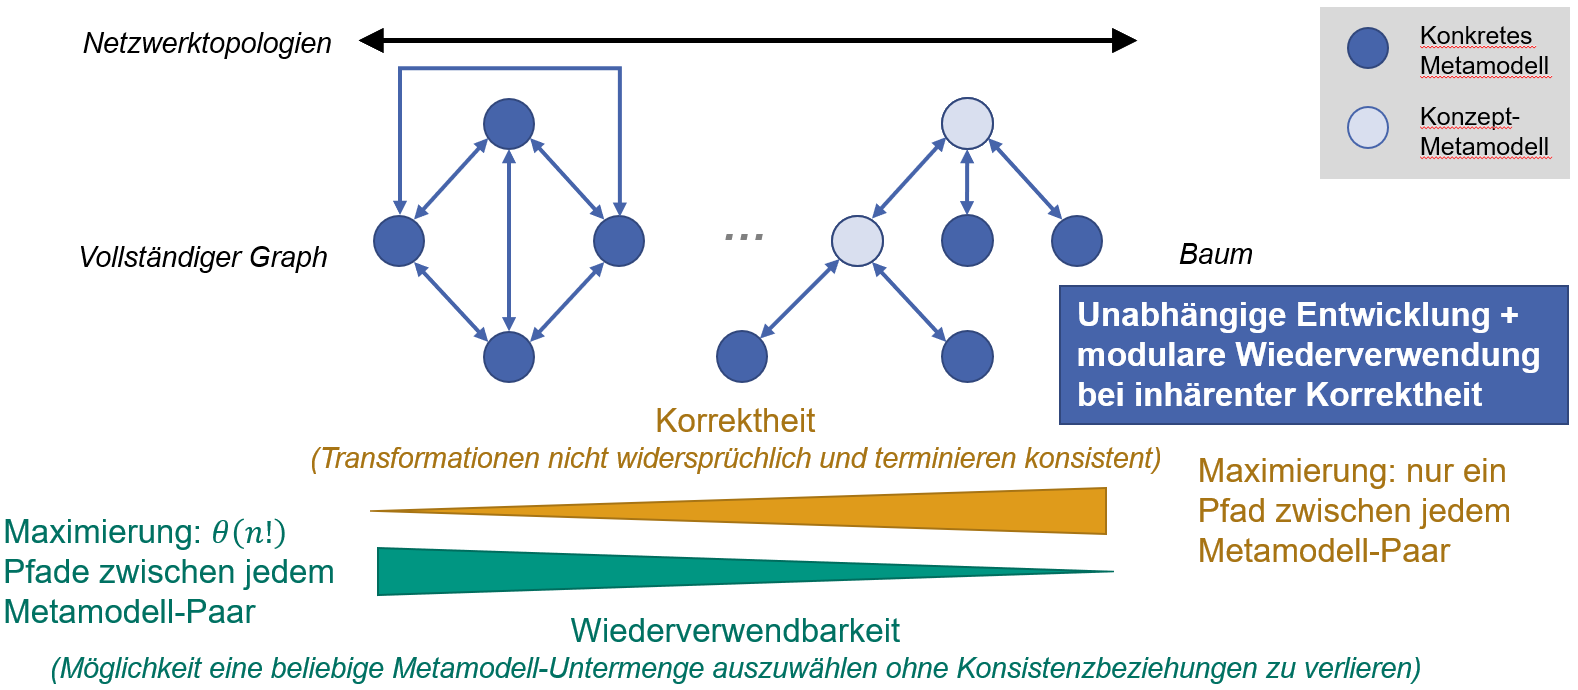
\includegraphics[width=\textwidth]{figures/quality/improvement/benefit_tradeoff.png}
%     \caption[Benefit of \commonalities regarding quality trade-offs]{Reduction of trade-off between quality properties using the \commonalities approach by ensuring correctness through a tree topology and achieving reusability by \concretemetamodels only being leaves.}
%     \label{fig:improvement:benefit_tradeoff}
% \end{figure}

% \todo{Instead of only discussion compatibility (which for sure is also true), discuss that in Commonalities there is always a consistent orchestration and that the shortest orchestration has an upper bound depending on the number of transformations. Discuss why this is not a drawback regarding such a bound in ordinary networks (especially discuss the previous example, where ping-pong was required, whereas here the required information is automatically added within the Commonalities and then only needs to be propagated back). However, there can still be scenarios that cannot be handled (due to the same reasons as for ordinary networks), but we already questioned there, although theoretically possible, whether they are practically relevant. In contrast to ordinary networks, Commonalities encode the limitation into the approach strategy and thus make it explicit for the developer rather then defining individual transformation without knowing how often they are executed later on. 
% -- Since the problem still remains, we did only discuss its mitigation already before}


\subsection{Reducing Specification Effort}
\label{chap:improvement:benefits:specification_effort}

\mnote{Redundancies in consistency relations}
While the mitigation of the trade-off between correctness and reusability of a transformation network through the use of the \commonalities approach represents its major benefit, it can also reduce specification effort.
This is achieved by the fact that each consistency relation must, in the best case, only be defined once, whereas in a transformation network inducing a dense or even complete graph, there need to be redundant representations of the same relations if arbitrary parts of the network are supposed to be reusable.

\begin{figure}
    \centering
    \newcommand{\classwidth}{5em}
\newcommand{\hdistance}{11em}
\newcommand{\innerhdistance}{10em}
\newcommand{\labeldistance}{1em}
\newcommand{\mmborder}{1em}


\begin{tikzpicture}[
    manifests relation label/.style={stereotype, above, sloped}
]

\pgfdeclarelayer{bg}
\pgfsetlayers{bg,main}

\umlclassvarwidth{network_java_class}{}{Class}{
    name\\
    packageName
}{\classwidth}

\umlclassvarwidth[, right=\hdistance of network_java_class.north, anchor=north]{network_uml_class}{}{Class}{
    name
}{\classwidth}
\umlclassvarwidth[, right=\innerhdistance of network_uml_class.north, anchor=north]{network_uml_package}{}{Package}{
    name
}{\classwidth}

\umlclassvarwidth[, below right=0.5*\hdistance and \hdistance of network_java_class.north, anchor=north]{network_c_class}{}{Class}{
    name\\
    namespace
}{\classwidth}

\umlcomposition{(network_uml_package) -- node[uml role end, pos=1, above right] {classes} node[uml cardinality end, pos=1, below right] {*} (network_uml_class.east|-network_uml_package.west)}

\node[mmlabel, above=\labeldistance of network_java_class.north, anchor=center] (network_java_label) {Java};
\node[mmlabel, anchor=center] (network_uml_label) at ([yshift=\labeldistance]$(network_uml_class.north)!0.5!(network_uml_package.north)$) {\acrshort{UML}};
\node[mmlabel, below=\labeldistance of network_c_class.south, anchor=center] (network_c_label) {\cplusplus};

\begin{pgfonlayer}{bg}
    \node[mmbg, fit=(network_java_class)(network_java_label.center), inner sep=\mmborder] (network_java) {};
    \node[mmbg, fit=(network_uml_class)(network_uml_package)(network_uml_label.center), inner sep=\mmborder] (network_uml) {};
    \node[mmbg, fit=(network_c_class)(network_c_label.center), inner sep=\mmborder] (network_c) {};
\end{pgfonlayer}

\draw[transformation] (network_java_class.east|-network_uml_class.west) -- node[stereotype, above] {«transforms»} (network_uml_class);
\draw[transformation] (network_java_class.south) |- node[stereotype, above, pos=0.75] {«transforms»} (network_c_class.west);
\draw[transformation] (network_uml_class) -- node[stereotype, right] {«transforms»} (network_c_class);



\umlclassvarwidth[, below right=1.45*\hdistance and \hdistance of network_java_class.north, anchor=north]{comm_oo_class}{}{Class}{
    name
}{\classwidth}

\umlclassvarwidth[, right=\innerhdistance of comm_oo_class.north, anchor=north]{comm_oo_package}{}{Package}{
    name
}{\classwidth}

\umlcomposition{(comm_oo_package) -- node[uml role end, pos=1, above right] {classes} node[uml cardinality end, pos=1, below right] {*} (comm_oo_class.east|-comm_oo_package.west)}

\umlclassvarwidth[, below left=0.65*\hdistance and \hdistance of comm_oo_class.north, anchor=north]{comm_java_class}{}{Class}{
    name\\
    packageName
}{\classwidth}

\umlclassvarwidth[, right=\hdistance of comm_java_class.north, anchor=north]{comm_c_class}{}{Class}{
    name\\
    namespace
}{\classwidth}

\umlclassvarwidth[, right=\hdistance of comm_c_class.north, anchor=north]{comm_uml_package}{}{Package}{
    name
}{\classwidth}

\umlclassvarwidth[, below=0.5*\innerhdistance of comm_uml_package.north, anchor=north]{comm_uml_class}{}{Class}{
    name
}{\classwidth}

\umlcomposition{(comm_uml_package) -- node[uml role end, pos=1, above right] {classes} node[uml cardinality end, pos=1, above left] {*} (comm_uml_class)}

\coordinate (comm_oo_label_coordinate) at ($(comm_oo_class.north)!0.5!(comm_oo_package.north)$);
\node[mmlabel, above=\labeldistance of comm_oo_label_coordinate, anchor=center] (comm_oo_label) {Object-oriented Design};
\node[mmlabel, below=\labeldistance of comm_java_class.south, anchor=center] (comm_java_label) {Java};
\node[mmlabel, below=\labeldistance of comm_c_class.south, anchor=center] (comm_c_label) {\cplusplus};
\node[mmlabel, below=\labeldistance of comm_uml_class.south, anchor=center] (comm_uml_label) {\acrshort{UML}};

\begin{pgfonlayer}{bg}
    \node[conceptmmbg, fit=(comm_oo_class)(comm_oo_package)(comm_oo_label.center), inner sep=\mmborder] (comm_java) {};
    \node[mmbg, fit=(comm_java_class)(comm_java_label.center), inner sep=\mmborder] (comm_java) {};
    \node[mmbg, fit=(comm_c_class)(comm_c_label.center), inner sep=\mmborder] (comm_c) {};
    \node[mmbg, fit=(comm_uml_class)(comm_uml_package)(comm_uml_label.center), inner sep=\mmborder] (comm_uml) {};
\end{pgfonlayer}

\draw[manifests relation] (comm_oo_class) -- node[manifests relation label] {\manifestslabel} (comm_java_class);
\draw[manifests relation] (comm_oo_class) -- node[manifests relation label] {\manifestslabel} (comm_c_class);
\draw[manifests relation] (comm_oo_class) -- node[manifests relation label] {\manifestslabel} (comm_uml_class);
\draw[manifests relation] (comm_oo_package) -- node[manifests relation label] {\manifestslabel} (comm_uml_package);


\node[above=3*\labeldistance of network_uml_class.north, anchor=center, font=\small\bfseries] {Transformation Network};
\node[above=3*\labeldistance of comm_oo_class.north, anchor=center, font=\small\bfseries] {\Commonalities Specification};

\end{tikzpicture}
    %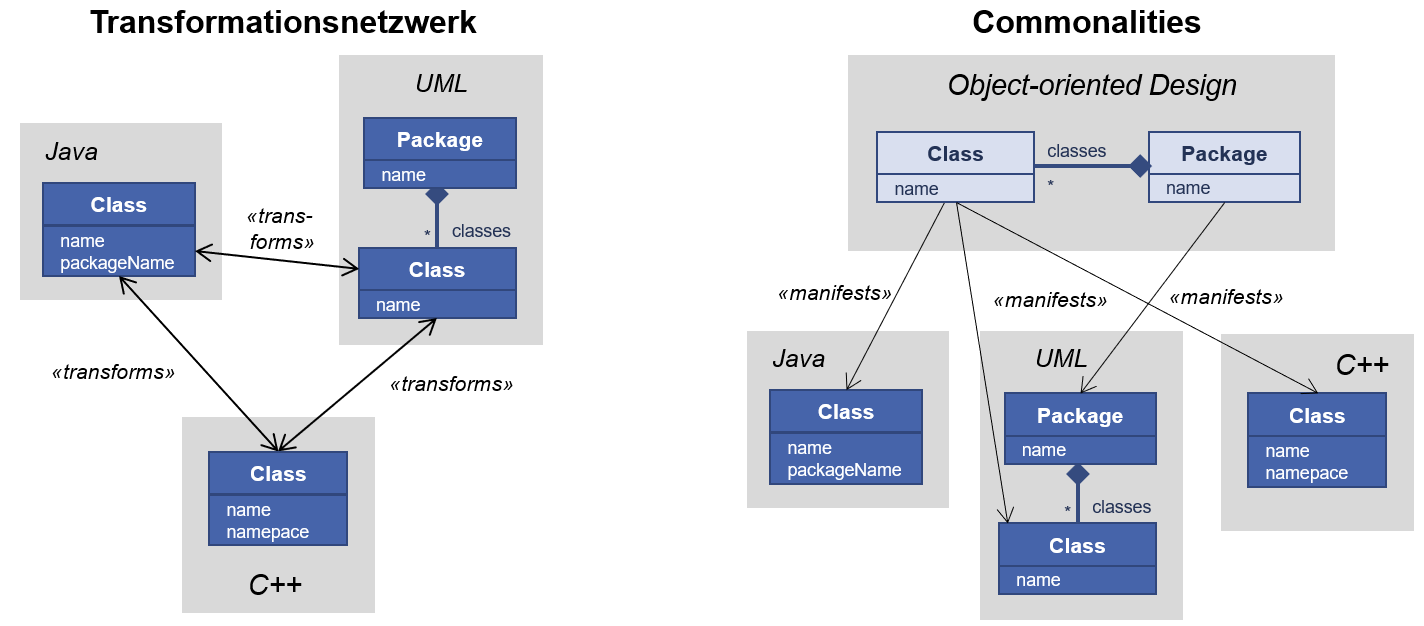
\includegraphics[width=\textwidth]{figures/quality/improvement/benefit_specification_effort.png}
    \caption[Benefit of \commonalities regarding specification effort]{Example for the number of defined relations with ordinary transformation networks and the usage of \conceptmetamodels with the \commonalities approach.} % affecting the specification effort.}
    \label{fig:improvement:benefit_specification_effort}
\end{figure}

\mnote{Specification example}
\autoref{fig:improvement:benefit_specification_effort} depicts an the extension of the introductory example given in \autoref{fig:improvement:running_example}, in which in addition to classes in \gls{UML} and Java a representation in \cplusplus is added.
In case of a transformation network, the relation between \cplusplus and both Java and \gls{UML} needs to be defined.
Using the \commonalities approach, only an additional manifestation relation to the concepts already defined in the object-oriented design \conceptmetamodels has to be specified.
In general, if $n$ metamodels share common concepts, adding an $n$-$1$-th metamodel requires $n$ transformations to be defined in ordinary networks, whereas the \commonalities approach, in the best case, only requires one addition manifestation relation to be defined.

\mnote{The average case}
The best case is, however, only achieved if the \conceptmetamodel already contains all information shared between the \concretemetamodel to be added and the ones for which the manifestation of the \commonalities in the \conceptmetamodel is already defined.
This is due to the already discussed fact that, informally speaking, the \conceptmetamodel needs to represent the union of all pairwise intersections of the \concretemetamodels.
Thus, usually it will be necessary to also extend or adapt the \conceptmetamodel and define or modify manifestations in the other \concretemetamodels as well.
For this scenario, a language that combines the specification of each \commonality with its manifestation relations, as we propose in \autoref{chap:language}, provides further benefits, as a modification or extension of a \commonality can be performed along with adaptations of the existing manifestation relations at one place.

\mnote{Initial effort}
In addition, applying the \commonalities approach may produce higher initial effort for the first consistency relations.
For two metamodels to keep consistent, one \conceptmetamodel and two manifestation relations have to be defined instead of only a single transformation in case of directly relating the two metamodels.
This initial effort amortizes only if enough further \concretemetamodels are kept consistent via the same \conceptmetamodel.

\mnote{Initial effort reduction}
The initial specification effort can, however, also be reduced by providing a specific language to define \commonalities, which combines the definition of manifestation relations with the definition of its \commonality, such that the specification becomes nearly as concise as it would be if defined as a direct consistency relation between two metamodels.
We propose such a language in \autoref{chap:language} and discuss this benefit in \autoref{chap:language:commonalities:benefits}.


% \begin{copiedFrom}{DocSym}

% This approach addresses all identified challenges % identified in \autoref{sec:approach:challenges} 
% and solves them under the assumption that all consistency relations %of a system 
% are described using \glspl{CMM}. %if their specification is encapsulated in a specialized language, our challenges identified in \autoref{sec:approach:challenges} can be addressed.
% %Under the assumption that all consistency relations of a system can be described using \acp{CMM}, we would be able to solve all identified challenges, as using \acp{CMM} allows to have the expressiveness of a graph of transformations, but abstracted to a tree structure with all its advantages.
% %We achieve \emph{uniqueness} by extracting common concepts into \acp{CMM} having to define only one relation of a metamodel to the \ac{CMM}. 
% We achieve inherent transformation compatibility by avoiding more than one transformation path %for the propagation of one change 
% between two metamodels by design. %Therefore, it is necessary to define \acp{CMM} relations in a way such that they induce a tree by also extracting common concepts of \acp{CMM} in other \acp{CMM}.  
% Since metamodels are only coupled across \glspl{CMM} and thus represent leaves of the transformation tree, any subset of them can be selected, maximizing modularity. % can be performed in a concrete usage scenario, maximizing modularity.
% %Finally, we assume that expressing consistency with explicit common concepts improves comprehensibility, %over combining binary consistency specifications
% %as it is a more natural representation and especially no transformations paths have to be traversed to understand a specific relation. % and expressing common information in common concepts is more natural than expressing it in transformations.
% %An approach of adding additional metamodels is also shortly discussed in~\cite{stevens2020BidirectionalTransformationLarge-SoSym}, but with the focus on definability of multiary relations rather than the optimization regarding certain challenges.
% Finally, we assume that making common concepts explicit improves comprehensibility.

% \end{copiedFrom} % DocSym

% \begin{copiedFrom}{VoSE}

% % BENEFITS
% We expect several benefits from our approach, i.e., specifying \commonalities, in comparison to direct transformation specifications between metamodels.
% First, we claim to achieve \emph{better understandability} of relations between metamodels, because common concepts are made explicit. % rather than encoding them implicitly in transformations.
% Second, the approach \emph{reduces errors} when more than two metamodels are to be kept consistent.
% Transformations usually relate two metamodels, especially because multidirectional relations are hard to express~\cite{stevens2020BidirectionalTransformationLarge-SoSym},
% %\modified{either because the developer does not know about multidirectional relations or due to cognitive limitations~\cite{stevens2020BidirectionalTransformationLarge-SoSym},} %keep instances of two metamodels consistent 
% and therefore have to be combined to a network of transformations to keep instances of more than two metamodels consistent.
% % Following sentence moved from approach section
% Such a network can be regarded as a graph, formed by metamodels as its nodes and transformations as its edges.
% However, such a network can easily raise compatibility problems if there exists more than one path of transformations between two metamodels.
% A hierarchy of \commonality specifications is, by design, not prone to such problems.
% Finally, we \emph{improve reusability} in comparison to a network of transformations, %regarding a network of transformations, 
% because an arbitrary subset of metamodels, between which \commonalities are defined, can be selected to keep their instances consistent.
% In contrast, removing metamodels from a transformation network can easily lead to missing transformation paths between two metamodels.

% Benefits:
% \begin{itemize}
%     \item \emph{Better understandability} of relations, as common concepts are explicitly defined rather than implicitly encoding them in transformations
%     \item \emph{Improved reusability / partial usability} (regarding networks of binary transformations), because an arbitrary selection of concrete metamodels can be used and kept consistent
%     \item \emph{High expressiveness}, because no restriction due to predefined sets of statements, as expression can be added dynamically. This can be also improve analyzability of transformations, as additional metadata could be defined for each of the extensions.
% \end{itemize}

% \subsection*{Benefits of \commonalities}
% \label{chap:commonalities:approach:benefits}

% We suppose the \commonalities approach to provide two kinds of benefits:
% First, we expect that it improves understandability of relations between metamodels, because common concepts are not encoded in transformations implicitly but modelled explicitly.
% This is even a benefit if instances of only two metamodels shall be kept consistent.
% Second, it reduces problems that can occur if several bidirectional transformations are combined into a network of transformations to keep multiple models consistent.

% Two types of benefits:
% \begin{itemize}
%     \item Independent from network size: Understandability (explicit commonalities rather than implicit encoding in constraints)
%     \item Benefits for transformation networks (in the following)
% \end{itemize}

% \begin{figure}
%     \centering
%     \begin{minipage}[b]{0.49\columnwidth}
%         \centering
%         \newcommand{\hmmdistance}{3.6em}
\newcommand{\vmmdistance}{2.4em}

\begin{tikzpicture}[
    mm/.style={schematic metamodel},
]

\node[mm] (full_left) {};
\node[mm, above right=\vmmdistance and \hmmdistance of full_left.center, anchor=center] (full_top) {};
\node[mm, below right=\vmmdistance and \hmmdistance of full_left.center, anchor=center] (full_bottom) {};
\node[mm, right=2*\hmmdistance of full_left.center, anchor=center] (full_right) {};
\node[mm, below left=\vmmdistance and \hmmdistance of full_left.center, anchor=center] (full_bottomleft) {};

\draw[transformation] (full_left) -- (full_top);
\draw[transformation] (full_left) -- (full_right);
\draw[transformation] (full_left) -- (full_bottom);
\draw[transformation] (full_top) -- (full_right);
\draw[transformation] (full_top) -- (full_bottom);
\draw[transformation] (full_right) -- (full_bottom);
\draw[transformation] (full_left) -- (full_bottomleft);
\draw[transformation] (full_bottom) -- (full_bottomleft);
\draw[transformation] (full_top) to[bend right=30] (full_bottomleft);
\draw[transformation] (full_bottomleft) .. controls ++(1*\hmmdistance, -0.8*\vmmdistance) and ([yshift=-1.5*\vmmdistance]full_right.south) .. (full_right);

\end{tikzpicture}
%         \subcaption{Dense Graph}
%         \label{fig:improvement:topologies:full}
%     \end{minipage}
%     \hfill
%     \begin{minipage}[b]{0.49\columnwidth}
%         \centering
%         \newcommand{\hmmdistance}{3.6em}
\newcommand{\vmmdistance}{2.4em}

\begin{tikzpicture}[
    conceptmm/.style={schematic conceptmetamodel},
    concretemm/.style={schematic metamodel},
]

\node[conceptmm, right=4*\hmmdistance of full_left.center, anchor=center] (tree_left) {};
\node[conceptmm, above right=\vmmdistance and \hmmdistance of tree_left.center, anchor=center] (tree_top) {};
\node[concretemm, below right=\vmmdistance and \hmmdistance of tree_left.center, anchor=center] (tree_bottom) {};
\node[concretemm, right=2*\hmmdistance of tree_left.center, anchor=center] (tree_right) {};
\node[concretemm, below left=\vmmdistance and \hmmdistance of tree_left.center, anchor=center] (tree_bottomleft) {};

\draw[transformation] (tree_left) -- (tree_top);
\draw[transformation] (tree_left) -- (tree_bottom);
\draw[transformation] (tree_left) -- (tree_bottomleft);
\draw[transformation] (tree_top) -- (tree_right);

\end{tikzpicture}
%         \vspace{1em}
%         \subcaption{Tree}
%         \label{fig:improvement:topologies:tree}
%     \end{minipage}
%     \caption[Extremes of transformation network topologies]{Extremes of transformation network topologies: nodes represent metamodels, edges represent transformations (\conceptmetamodels in a tree of \commonalities in dark gray). Adapted from~\owncite[Fig. 4]{klare2019models}.}
%     \label{fig:improvement:topologies}
% \end{figure}

% Networks of transformations can have two extremes of topologies, as depicted in \autoref{fig:improvement:topologies}.
% If transformations between all metamodels are defined, the network forms a dense graph (see \autoref{fig:improvement:topologies:full}).
% In contrast, if there exists exactly one path of transformations between each pair of metamodels, the network forms a tree (see \autoref{fig:improvement:topologies:tree}).
% Several properties for such %transformation 
% networks have been identified by \textcite{gleitze2017a} and \textcite{klare2018docsym}.
% Two essential properties %, defined in~\cite{klare2018docsym}, 
% are \emph{compatibility} and \emph{modularity}~\cite{klare2018docsym}, which, unfortunately, contradict each other.
% The \commonalities approach, however, improves both of them. %, which is an essential benefit that we discuss in the following. %We discuss the benefits of the \commonalities approach regarding those properties.
% \emph{Compatibility} means that transformations do not define contradictory constraints.
% Consider the relations introduced for the running example in \autoref{fig:improvement:running_example}.
% The names of the same class in Java and UML are defined to be equal.
% If a class in Java and UML realizes a \gls{PCM} component, it shall have the same name appended with an \enquote{Impl} suffix.
% If transformations realize the three relations between \gls{PCM}, UML and Java, and the one between \gls{PCM} and Java adds that suffix whereas the one between \gls{PCM} and UML omits it, the constraints can never be fulfilled.
% %If the three relations between Java, UML and \ac{PCM} are defined in transformations and the one between \ac{PCM} and Java adds that suffix whereas the one between \ac{PCM} and UML omits it, the constraints can never be fulfilled.
% In that case, the transformations are considered incompatible.
% Incompatibility may arise whenever more than one transformation path between two metamodels exists.
% In consequence, compatibility cannot be guaranteed in dense network, whereas it is inherently high if the network forms a tree.
% \emph{Modularity} means that any subset of the metamodels can be used without loosing consistency because of missing transformations.
% Modularity is high if any metamodel can be removed from the network and the remaining transformations still define consistency between all remaining metamodels.
% In consequence, modularity is high in a dense network, because all metamodels are directly related, while it is low if the network is a tree, because inner nodes cannot be removed without their children not being related by a transformation anymore.
% Since redundant paths between metamodels improve modularity but reduce compatibility, these properties are inherently contradicting.

% The \commonalities approach improves both these properties due to the fact that additional metamodels are introduced in the specification.
% The transformations between \metaclasses in \concretemetamodels and \commonalities in \conceptmetamodels induce a tree, thus compatibility is high.
% Additionally, only the leaves of the tree are \concretemetamodels, which are actually used to describe a system and whose instances are modified, whereas the inner nodes only represent auxiliary metamodels, exemplarily marked in \autoref{fig:improvement:topologies:tree}. 
% In consequence, taking an arbitrary subset of \concretemetamodels removes only leaves and can thus be done without removing any transformations that are necessary to keep instances of the remaining metamodels consistent.
% This constitutes a major benefit of the \commonalities approach as compared to ordinary networks of transformations.


% \subsection{Limitations of \commonalities}
% \label{sec:approach:limitations}
% ONE PART MOVED TO COMPOSITION (DAG INSTEAD OF TREES), ONE MOVED TO LIMITATIONS IN EVALUATION SECTION

% \end{copiedFrom} % VoSE

